\documentclass[a4paper,10pt]{article}

% Hier die Nummer des Blatts und Autoren angeben.
\newcommand{\blatt}{8}
\newcommand{\autor}{Ralf Engelken, Joachim Schmidberger, Frank Woithe, Michael Steinke, Merlin Koglin}

\usepackage{hci}
\usepackage{float} 

\begin{document}
% Seitenkopf mit Informationen
\kopf
\renewcommand{\figurename}{Figure}

\aufgabe{13 \textit{(Team-Aufgabe)}} 
Wählen Sie aus den folgenden Anwendungsdomänen jeweils ein konkretes interaktives System aus und beschreiben Sie das Konzeptionelle Modell dahinter. Konkretisieren Sie dies, indem Sie mindestens drei Interface-Elemente (pro System) auswählen und die dahinter stehende Metapher erklären. \newline
 
\textbf{\textit{1. eCommerce/Web-Shop (z.B. Amazon, Zalando, ...)}} \newline
Als Beispiel für einen Web-Shop soll hier \textbf{\textit {Pearl.de}} dienen. Die Seite wirkt sehr unaufgeräumt, eher wie die Reste-Box eines Geschäfts. Das Motto steht oben links, direkt unter dem Start-Logo: Immer preiswert und innovativ. Die Ware ist entsprechend zusammengestellt: Möglichst viel Funktionalität für wenig Geld, aber es muss nicht unbedingt hochwertig sein. Dem entsprechend werden auch gleich auf der Startseite möglichst viele Produkte angepriesen.\\
Dem konzeptionellen Modell des Web-Shop Interfaces soll vermutlich der reale Einkauf als Vorbild dienen, bei dem ein Kunde mit dem Einkaufswagen durch Regalreien schlendert, und hier und da mal etwas in seinen Einkaufswagen wirft.

\begin{figure}[H]
\centering 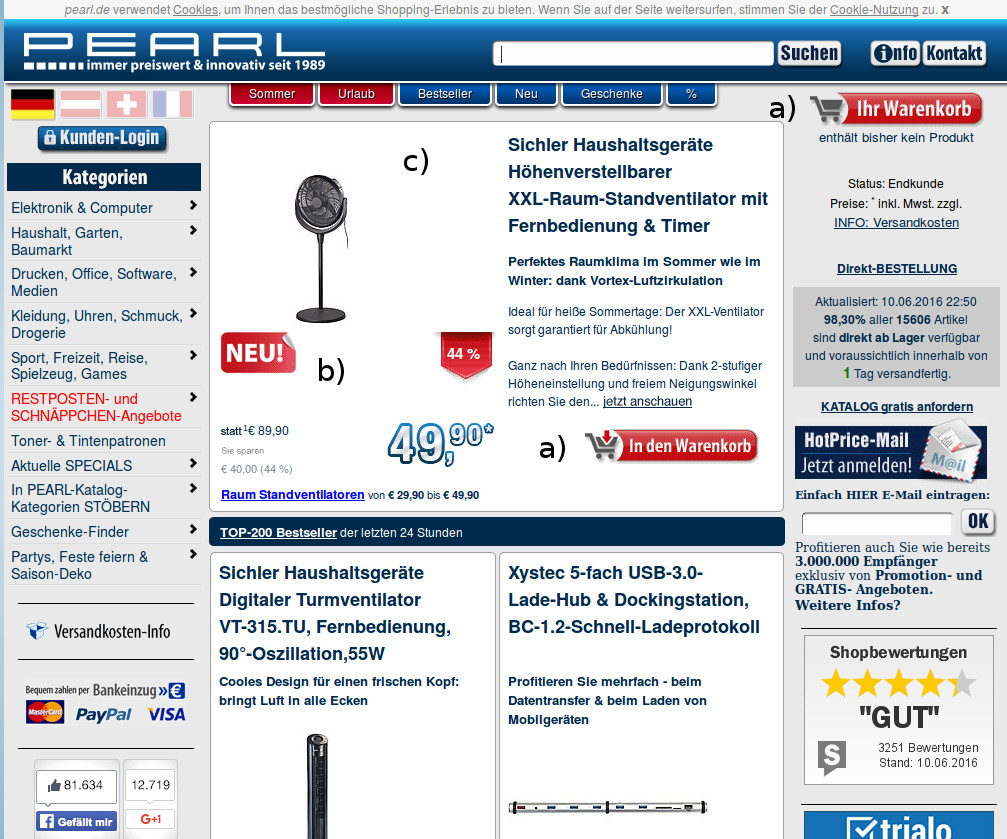
\includegraphics[width=1\textwidth]{pearl.jpg}
\caption{Navigations-Metaphern auf Pearl.de: a) Einkaufswagen, b) Neu - Aufkleber c) Obere Menuzeile}
\end{figure}

Bei der Suche nach Navigations Metaphern des Webshops sind mir folgende Elemente Aufgefallen:\newline
\begin{enumerate}
\item Pearl benutzt wie viele Web-Shops die Einkaufswagen-Metapher, welche mittlerweile zu einem Standard geworden ist. Zusätzlich wird das Ikon, durch einen roten Pfeil ergänzt, bei jedem Produkt verwendet. Dies soll an den realen Vorgang erinnern, Produkte in einen Einkaufswagen zu werfen. Die Interface-Gestallter erhoffen sich hier eine virtuelle Affordance zum Klick auf das Ikon.
\item Bewusst auffällig sind die zusätzlichen Aufkleber-Ikons bei verschieden Produkten. Sie sollen an einen roten Aufkleber erinnern, wie er in manchen realen Geschäften, z.B. bei reduzirter Ware, nachträglich aufgeklebt wird. Es handelt sich hier um einen Skeuomorphismus, der durch eine angedeutete, umgeknickte Ecke der Aufkleber unterstrichen wird. Allerdings ist dieser Stiel bei den restlichen Elementen nicht konsequent durchgehalten, was die Seite uneinheitlich wirken lässt.
\item Ein weiteres, auffälliges Bedienelement ist die horizontale, zentrale Menuleiste im Kopfteil der Seite. Sie wirkt wie heraushängende Laschen und vermittelt nicht die Affordance auf sie zu klicken, sondern eher, daran zu ziehen. Auch die verschiedenen Farben wirken eher irritierend.
\end{enumerate}

Zusammenfassend kann man die Seite weder als besonders stilsicher, konsequent noch ästhetisch gelungen bezeichnen. Dennoch scheint sie für ihre Zielgruppe zu funktionieren.\\

\textbf{\textit{2. Mediaplayer (um Audio oder Video Dateien abzuspielen)}} \newline

LORUM IPSUM ... \newline

\textbf{\textit{3. soziales Netzwerk}} \newline

Soziale Netzwerke versuchen konzeptionell kommunikationsbereiche eines Menschen in einem Netzwerk abzubilden. Dabei bedienen Sie sich an der "öffentlichkeit" der Kommunikation, also ob diese
\begin{enumerate}
\item zwischen zwei oder mehreren bekannten Menschen (z.B. Gruppennachrichten die eine direkte Konversation nachbilden können)
\item in einer offenen oder geschlossenen Gruppe, in der sich nicht jeder kennt oder(Forum oder Gruppen, die eine Konversation in einem Verein nachbilden können)
\item ungerichtet und dabei zwischen dem Individuum und allen bekannten und unbekannten (z.B. eine Nachricht an unbekannte über einen Zettel an der Staße (Suche Wohnung ect. pp))
\end{enumerate}

stattfindet. \newline

Ein Beispiel für ein soziales Netzwerk ist \textbf{\textit Facebook}, welches jedoch noch mehr Konzepte auf seiner Plattform mit dem kommunikations-Konzept verknüpft. Im Folgenden soll es nur um die Kommunikation gehen.

\begin{figure}[ht]
\centering 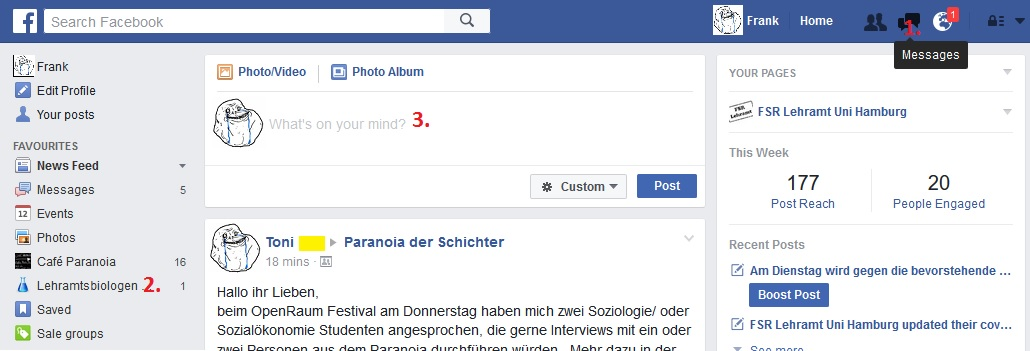
\includegraphics[width=1\textwidth]{facebook.jpg}
\caption{Navigations-Metaphern auf Facebook: 1. Nachrichten, 2. Symbol für eine (geschlossene) Gruppe, 3. die Pinnwand mit den Öffentlichkeitseinstellungen}
\end{figure}

Das Nachrichtensymbol (1) besteht aus zwei ineinander verschachtelten Sprechblasen. Sprechblasen werden oft als graphisches Mittel eingesetzt, um Gespräche zu symbolisieren. Das Symbol ist also eine Methaper für ein Gespräch zwischen zwei oder mehreren Personen. \newline
Die Metapher für eine Gruppe, in dem Fall die Gruppe 'Lehramtsbiologen' (2), besteht aus einem Reagenzglas und dem Text. An einem passenden Icon und dem Text soll der User erkennen um welche Art von Gruppe es sich handelt und auf dieses Klicken um den den Inhalt der Gruppe anzuzeigen. Fährt der User mit der Maus über die Gruppe, so wird sie etwas grauer hinterlegt, was einen Link oder klickbares Element andeutet. \newline
Die Pinnwand (3) trägt den Namen der Methapher schon in sich, denn sie soll wie eine Pinnwand im richtigen Leben fungieren. Je nachdem wo diese Pinnwand hängt (z.B. in einem abgeschlossenem Raum oder sichtbar zur Straße hin) sehen mehr oder weniger Menschen eine Nachricht auf dieser. Gleiches gilt auch hier: Der user schreibt eine Nachricht auf seine Pinnwand und "postet" diese. Über den Button "Custom" kann er noch einstellen, wer diese Nachricht sehen kann. \newline


\textbf{\textit{4. ein Programm/Website aus einer beliebigen weiteren Anwendungsdomäne}} \newline

LORUM IPSUM ... \newline


\end{document}
